\documentclass[10pt,a4paper]{article}
\linespread{1.5}

\usepackage[T1]{fontenc}
\usepackage{amsfonts}
\usepackage[utf8]{inputenc}
\usepackage{graphicx}
\usepackage{url} % príkaz \url na formátovanie URL
\usepackage{hyperref} % odkazy v texte budú aktívne (pri niektorých triedach dokumentov spôsobuje posun textu)
\setlength{\parindent}{0pt}
\newcommand{\parindentplus}{\hspace*{\parindent}\vspace{0em}}
\usepackage{cite}
\usepackage{multirow}

\pagestyle{headings}

\title{Ensuring Data Integrity and Reliability in Big Data\thanks{Semestrálny projekt v predmete Metódy inžinierskej práce, ak. rok 2023/24, vedenie: Mirwais Ahmadzai}}

\author{Michal Zrutta \\[2pt]
	{\small Slovenská technická univerzita v Bratislave}\\
	{\small Fakulta informatiky a informačných technológií}\\
	{\small \texttt{xzrutta@stuba.sk}}
}
\date{\small 5. November 2023}
\begin{document}

\maketitle

\begin{abstract}
\parindentplus We live in the era of Big Data.These days data comes too fast and in an enormous sizes, this requires better understanding of data and processing. Data generation increased by 95 zettabytes between 2010 and 2022.\\ \parindentplus However, the upward trajectory poses challenges in data quality. Consequently, the demand for realistic data sets, accurate and consistent information, and overall data quality has become a pressing concern.\\ \parindentplus This study delves into the challenges of data quality assurance in the realm of Big Data analytic, exploring methodologies to validate diverse and extensive data-sets. The research is shown on a context of gas consumption in various car models.\\ \parindentplus The paper later shows potential but already used integration of Artificial Intelligence. AI algorithms are supposed to identify and rectify inaccuracies, while also learning from the data to continuously enhance data quality.
\end{abstract}
\section{Introduction}
\subsection{Background}
In recent times, the term "Big Data" has become widespread, describing a massive amount of information flooding businesses, organizations, and research institutions daily. Big Data includes data-sets that are too large, complex, or fast-moving for regular data processing tools. Data comes from various sources like social media, sensors, online transactions, and multimedia. What makes Big Data unique isn't just its enormous size but also its speed, diversity, and reliability.\cite{gudivada2015big}
The rapid growth and widespread use of Big Data technologies have transformed industries and research fields globally. With the increasing digitization of information and advancements in data processing capabilities, organizations now have the ability to collect, store, and analyze massive volumes of data in real-time. This growth has been driven by the need to extract valuable insights, improve decision-making processes, enhance customer experiences, and gain competitive advantages. Industries ranging from business and health-care to science and social sciences have embraced Big Data technologies, leading to their everywhere use in diverse applications.\cite{anisetti2023assurance}
This requires accurate and precise data analysis to extract valuable insights, ensuring its usefulness across a wide range of industries. Trustworthiness in dealing with Big Data is really important. It means the information used is reliable and accurate, preventing mistakes. It also builds people's confidence and protects their privacy in our data-driven world.\cite{anisetti2023assurance}
\subsection{Problem Statement}
Big data analysis can transform raw data collected from users in a big data program into useful information. Wrong data and incorrect inputs can significantly alter the overall results, which are crucial in many cases. There are many works out there on data reliability. For example, consider buying a new laptop. You can rely on the specifications provided for the product. However, you also seek user experiences by reading comments. If there are many positive comments, you may feel confident about the purchase. But this system lacks credibility in verifying the trustworthiness of the person who wrote the comment. The question still remains: How can we ensure data quality?
\begin{itemize}
  \item Data Validity: Is the data fulfilling its intended purpose?
  \begin{itemize}
    \item Apple is a fruit, but it is also a company
  \end{itemize}
  \item Data Completeness/Accuracy: Is the data reliable for organizational use?
  \begin{itemize}
      \item Does all processed data necessary for decision-making exist?
      \item Can we trust the data used for calculations?
      \end{itemize}
  \item Data Consistency: Is the data consistent in its behavior?
  \begin{itemize}
    \item Apple is a fruit, but it is also a company
  \end{itemize}
\end{itemize}



\section{Previous Studies on Data Quality in Big Data}
\subsection{Data Accuracy and Reliability Evaluation for Big Data}
In the proposed data quality assessment process for big data, as outlined by Li Cai from Yunnan University, the initial step involves defining data collection goals aligned with strategic objectives. Users choose data based on factors like operations, decision-making, and planning. Quality elements vary with business environments; for example, social media data prioritize timeliness and credibility.
\\Specific dimensions, indicators, and assessment criteria are determined for each business context. Data cleaning is crucial for error detection and removal, enhancing data quality. The data acquisition phase employs various methods such as integration, search-download, and web crawlers.
\begin{figure*}[htbp]
  \centering
  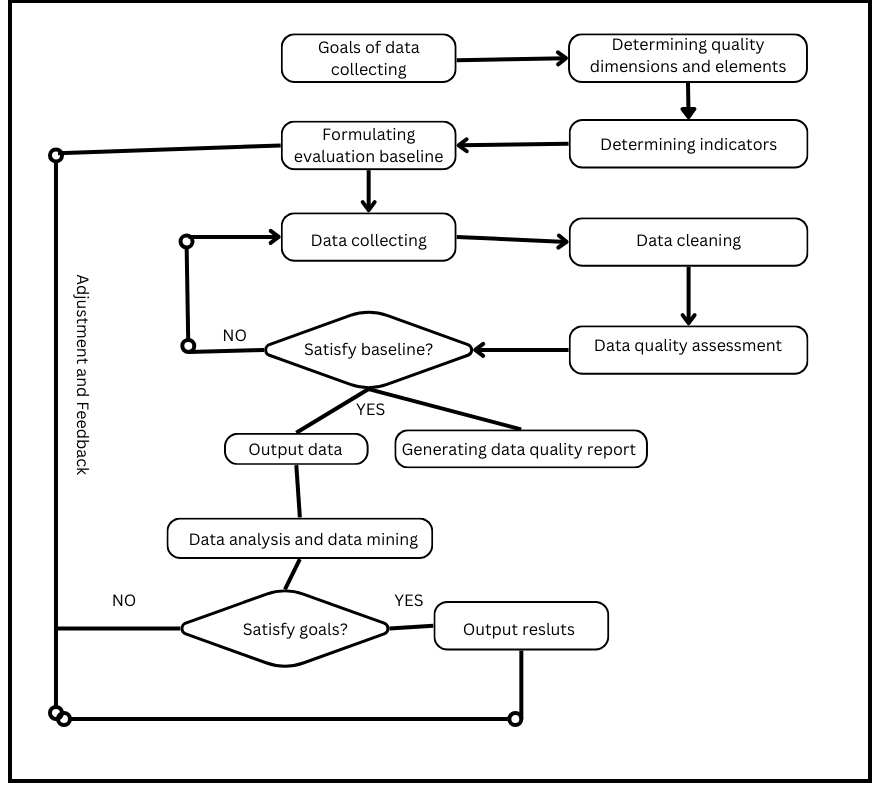
\includegraphics[width=0.8\columnwidth]{Quality assesment process for Big Data.png}
  \caption{Quality assessment for big data}
  \label{fig:quality-assessment}
\end{figure*}
\\ 
Following data collection, the paper emphasizes the importance of data cleaning to address issues like errors and inconsistencies. The assessment then enters qualitative and quantitative evaluation phases. If data quality meets the baseline standards, analysis proceeds, generating quality reports. Otherwise, adjustments are made, and new data acquisition may be necessary.
\\
While data analysis and mining aren't directly part of quality assessment, they play a vital role in dynamic adjustment and feedback. Successful analyses feed back into the quality assessment system, supporting continuous improvement. Adjustments are made if analysis results don't align with goals, ensuring an iterative and adaptive data quality assessment process.\cite{article}

\subsection{Semantic Integrity Analysis for Unstructured Big Data}
This study is dedicated to the evaluation of unstructured Big Data, focusing on a assessment process for unstructured datasets. The model show us several essential components that collectively contribute to the comprehensive evaluation of data quality, resulting in a detailed quality assessment report.
\begin{enumerate}
\item \textbf{Quality Requirements:} The process initiates with defining precise quality requirements aligned with the strategic objectives, ensuring that the assessment is tailored to meet specific business goals.
\item \textbf{Data Sources:} Unstructured data is diverse and originates from varied sources. Evaluating its quality necessitates a clear understanding of these sources, encompassing social media, sensors, multimedia, and other channels.
\item \textbf{Data Quality Repository:} A centralized repository is established to store and manage data quality-related information, facilitating seamless tracking and analysis.
\item \textbf{Sampling and Profiling:} The data undergoes sampling and profiling, enabling a deeper understanding of its characteristics and patterns, which is fundamental for quality evaluation.
\item \textbf{Preparation Process for Quality Evaluation:} Preparing the data for evaluation involves preprocessing steps to ensure consistency and completeness, laying the foundation for accurate assessment.
\item \textbf{Feature Selection and Quality Mapping:} Relevant features are meticulously selected, and quality mapping techniques are applied, allowing for a focused evaluation process and ensuring that quality assessment aligns with the specific attributes of unstructured data.
\item \textbf{Quality Assessment:} Utilizing both qualitative and quantitative methods, the data undergoes a rigorous evaluation. Qualitative analysis conducted by experts evaluates data based on specific criteria, while quantitative methods provide objective insights.
\end{enumerate}
\cite{8605945}
\subsection{AI and Crowdsourcing Solutions}
In this study, they demonstrate how AI can assist in managing Big Data lakes and handling diverse data from various sources, addressing challenges such as incomplete data, invalid entries, and uncertainties.
AI and crowsdsourcing can be used in this problem. AI is able to remove duplicates from database or knowledge base. And there are continuous studies in data quality.\cite{6949519}


\section{Methodology}
In crafting the methodology for this article, a comprehensive examination of existing literature and research on the subject of ensuring data quality served as the foundation. Different perspectives and approaches from various articles and studies paved the way for the innovation of a novel approach to address the challenges of data quality in the context of Big Data. The key steps of the developed methodology are outlined below:
\begin{enumerate}
    \item \textbf Literature Review
    \item \textbf Understanding the problem
    \item \textbf Identification of similar approaches
    \item \textbf Innovation through Integration
    \item \textbf Validation through a hierarchical data quality standard
\end{enumerate}
Through the systematic execution of these steps, the resulting methodology not only builds upon the wealth of existing knowledge but also introduces a fresh perspective that is responsive to the evolving landscape of Big Data.

\begin{table}[]
\small % Adjust the font size if needed
\begin{tabular}{|l|l|l|}
\hline
Dimensions                                                     & Elements      & Indicators                                                                                                                                                                                                                                                         \\ \hline
\multirow{2}{*}{Availability}                                  & Accessibility & \begin{tabular}[c]{@{}l@{}}Whether a data access interface is provided\\ Data can be easily made public or easy to purchase\end{tabular}                                                                                                                           \\ \cline{2-3} 
                                                               & Timeliness    & \begin{tabular}[c]{@{}l@{}}Within a given time, whether the data arrive on time\\ Whether data are regularly updated\\ Whether the time interval from data collecion\\ and processing to release meets requirements\end{tabular}                                   \\ \hline
Usability                                                      & Credibility   & \begin{tabular}[c]{@{}l@{}}Data come from specialized organizations of a country, \\ field, or industry\\ Experts or specialists regularly audit and check \\ the correctness of data content\\ Data exist in the range of known or acceptable values\end{tabular} \\ \hline
\multirow{4}{*}{Reliability}                                   & Accuracy      & \begin{tabular}[c]{@{}l@{}}Data provided are accurate\\ Data representation (or value) well reflects the\\ true state of the source information\\ Information (data) representation will not be equivocal\end{tabular}                                             \\ \cline{2-3} 
                                                               & Consistency   & \begin{tabular}[c]{@{}l@{}}After data have been processed, their concepts, value\\ domains, and formats still match as before processing\\ During a certain time, data remain consistent\end{tabular}                                                              \\ \cline{2-3} 
                                                               & Integrity     & \begin{tabular}[c]{@{}l@{}}Data format is clear and meets the criteria\\ Data are consistent with structural integrity\\ Data are consistent with content integrity\end{tabular}                                                                                   \\ \cline{2-3} 
                                                               & Completeness  & \begin{tabular}[c]{@{}l@{}}Whether the deficiency of a component will impact use\\ of the data with multi-components\\ Whether the deficiency of a component will impact\\ data accuracy and integrity\end{tabular}                                                \\ \hline
Relevance                                                      & Fitness       & \begin{tabular}[c]{@{}l@{}}The data collected do not completely match the theme,\\ but they expound one aspect\\ Most datasets retrieved are within the retrieval\\ users need\\ Information theme provides matches with\\ users retrieval theme\end{tabular}      \\ \hline
\begin{tabular}[c]{@{}l@{}}Presentation\\ Quality\end{tabular} & Readability   & \begin{tabular}[c]{@{}l@{}}Data (content, format, etc.) are clear and understandable\\ It is easy to judge that the data provided meed need\\ Data description, classification, and coding content\\ satisfy specification and are easy to understand\end{tabular} \\ \hline
\end{tabular}
\caption{The hierarchical big data quality assessment framework}
\end{table}

\subsection{Proposed Methodology for Data Quality Assurance in Big Data}
If we had to collect data from all specific car model in the world for particular information, for example gas consumption.
Firstly we would need to specify:
\begin{enumerate}
    \item \textbf{Where?} It is really important where the car is driven. If it is somewhere rainy, for example Britain, or in Australia where it is hot, or in Canada where it is cold. The car and it's use is totally different and collected data which are not selected correctly would result in not proper product. For example electric cars like Tesla have difficulties in cold environment.
    \item \textbf{Who?} Everybody drives their cars differently so in order to get good results we need drivers who have similar driving skills.
    \item \textbf{When?} The time of data collection is crucial. Gas consumption can vary based on the time of day, traffic conditions, and seasons. For instance, in urban areas, gas consumption might differ during rush hours compared to non-peak times. Similarly, seasonal variations, such as summer and winter, can impact a car's fuel efficiency. Collecting data over different times and seasons can provide a comprehensive understanding of gas consumption patterns.
\end{enumerate}
Secondly, I recommend implementing a user ranking system for data contributors. Because if he is not qualified as a driver who has driving style as we need. For example, if a participant drives their car in a desert, which is vastly different from the study's target environments, their data might not be suitable for the overall analysis.\cite{8605945}
\\Once the data is collected from verified users we have to clean them and sort them out.
As we can see in previous study we can use AI to help us clear and clean data to enhance data accuracy. AI can automatically identify and correct mistakes. \\Additionally, AI possesses a deep understanding of physics, enabling it to perform calculations to validate the data accuracy and identify errors. \\Moreover, AI systems incorporate self-learning mechanisms, allowing them to learn from the collected data. This self-learning capability ensures continuous improvement in data quality over time by learning from past mistakes and refining its algorithms for future analyses.\cite{6949519}


\section{Objectives}
This paper aims to explore strategies ensuring data quality within the realm of Big Data. By addressing the challenges associated with incorrect data and not verified data it proposes methodologies to validate data quality. Through these strategies, the paper seek to help sort and clean data for reliable, accurate, and trustworthy data analysis in the era of Big Data.

\section{Results}

In this section, we present a summary of the results obtained from the application of our proposed methodology for data quality assurance in the context of gas consumption data from various car models.



\subsection{Data Collection and Selection}

The data collection process focused on obtaining information about gas consumption in specific car models under varying conditions. Key aspects considered during data collection included geographical location, driver qualifications, and the timing of data collection.

\subsubsection{Geographical Considerations}

The geographical location of the data collection significantly influenced the results. For example, cars driven in colder climates exhibited different gas consumption patterns compared to those in warmer environments. This emphasizes the importance of considering the location factor in data selection.

\subsubsection{Driver Qualifications}

The user ranking system implemented for data contributors played a crucial role in ensuring the quality of the collected data. Drivers with similar driving styles were prioritized, leading to a more homogeneous data-set.

\subsubsection{Timing of Data Collection}

Variations in gas consumption based on the time of day, traffic conditions, and seasons were evident in the collected data. This highlights the importance of capturing data over different times and seasons to obtain a comprehensive understanding of gas consumption patterns.

\subsection{Data Cleaning and AI Integration}

Following data collection, the integration of artificial intelligence (AI) proved instrumental in enhancing data accuracy and reliability. The AI system automatically identified and corrected errors, leveraging its understanding of physics and self-learning mechanisms. This resulted in a more refined data-set suitable for analysis.

\subsection{Analysis of Gas Consumption Patterns}

The processed data was subjected to analysis to identify patterns in gas consumption across different car models. The results provided insights into factors influencing gas consumption, including driving conditions, vehicle specifications, and environmental variables.

\section{Conclusion}

The application of the proposed methodology showcased its effectiveness in ensuring data quality in the realm of gas consumption data from various car models. The combination of careful data selection, AI-based data cleaning, and thorough analysis contributed to the reliability and accuracy of the results.

In conclusion, our research highlights the importance of a systematic approach to data quality assurance in the era of Big Data, particularly when dealing with diverse data-sets such as gas consumption in the automotive industry.

\bibliographystyle{abbrv}
\bibliography{citations}
\end{document}